\documentclass[tikz,border=10pt]{standalone}
\usepackage{helvet}
\renewcommand{\familydefault}{\sfdefault}
\usepackage{tikz}
\usetikzlibrary{arrows.meta, positioning, fit, calc, shapes.geometric, decorations.pathreplacing}

\definecolor{emeraldpine}{HTML}{1A4D3E}
\definecolor{ethbronze}{HTML}{B87333}
\definecolor{ethpetrol}{HTML}{007A87}
\definecolor{softink}{HTML}{4A5568}
\definecolor{ink}{HTML}{1A202C}

\definecolor{brainbg}{HTML}{F7EDE3}
\definecolor{structbg}{HTML}{E8F0EC}
\definecolor{worldbg}{HTML}{E3F3F5}
\definecolor{cardbg}{HTML}{F8FAFC}

\begin{document}
\newcommand{\titlefont}{\sffamily\bfseries\fontsize{10.5}{12}\selectfont\color{ink}}
\newcommand{\subfont}{\sffamily\fontsize{8.5}{10}\selectfont\color{softink}}

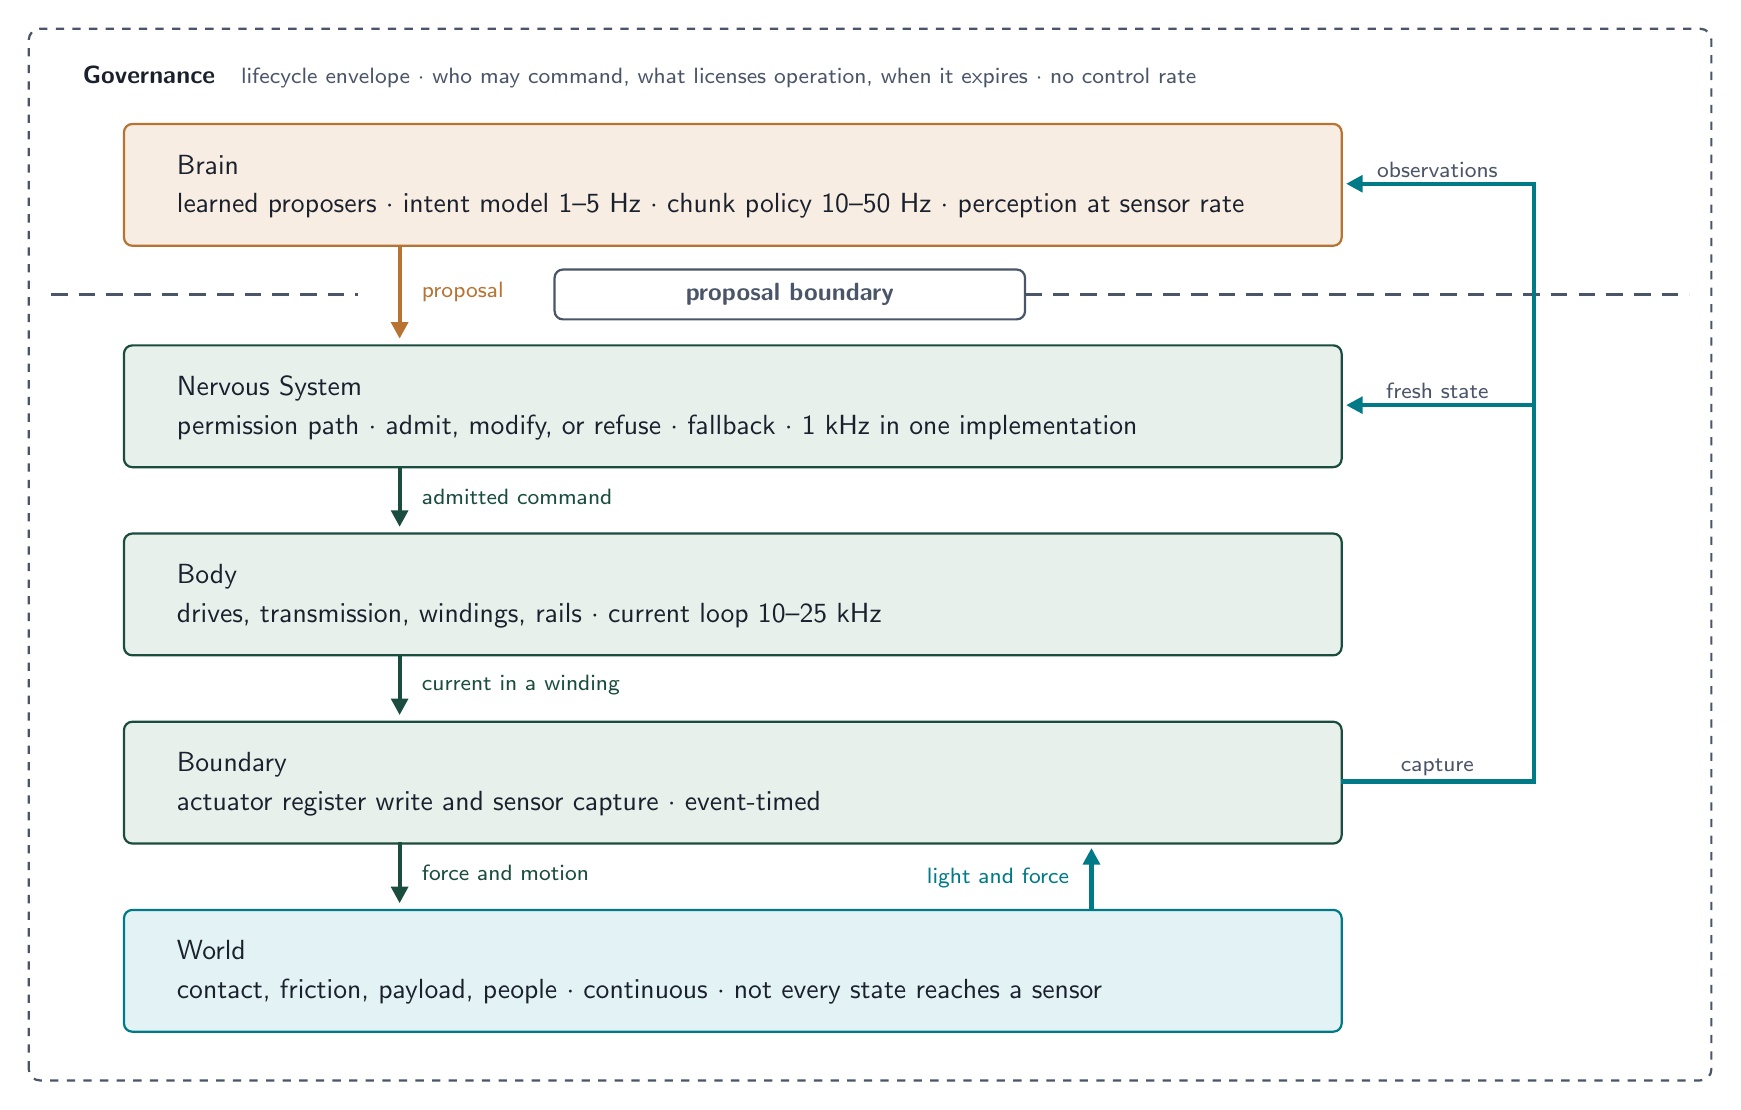
\begin{tikzpicture}[
    x=1pt, y=1pt, % Use point coordinates roughly matching SVG for easy layout
    >=stealth,
    tier/.style={
        draw, thick, rounded corners=3pt,
        minimum width=440pt, minimum height=44pt,
        align=left, inner xsep=16pt, inner ysep=0pt,
        anchor=north west
    },
    tiertext/.style={
        anchor=north west,
        font=\sffamily\color{ink},
        text width=410pt
    },
    arr-proposal/.style={->, thick, ethbronze, line width=1.5pt},
    arr-struct/.style={->, thick, emeraldpine, line width=1.5pt},
    arr-measure/.style={->, thick, ethpetrol, line width=1.5pt},
    arrlabel/.style={
        font=\sffamily\fontsize{8.5}{10}\selectfont\color{softink},
        anchor=west
    }
]

% Governance Box
\draw[softink, thick, dashed, rounded corners=4pt] (36, -396) rectangle (644, -16);
\node[anchor=north west] at (52, -26) {
    \textbf{\fontsize{9.5}{11}\selectfont\color{ink}Governance}\hspace{6pt}
    \fontsize{8.5}{10}\selectfont\color{softink}lifecycle envelope $\cdot$ who may command, what licenses operation, when it expires $\cdot$ no control rate
};

% Proposal Boundary
\draw[softink, thick, dash pattern=on 6pt off 4pt] (44, -112) -- (155, -112);
\draw[softink, thick, dash pattern=on 6pt off 4pt] (396, -112) -- (636, -112);
\node[fill=white, draw=softink, thick, rounded corners=3pt, minimum width=170pt, minimum height=18pt, anchor=center] 
    at (311, -112) {\fontsize{9}{11}\selectfont\itshape\color{softink}\bfseries proposal boundary};

% Tiers (Anchor at north-west coordinates matching SVG roughly)
% Y coordinates are negative because tikz standard is Y-up, SVG is Y-down.
% To map SVG y to TikZ y, we can just use y=-SVG_Y
% SVG coordinates:
% Brain: (70, 50)
% Nervous System: (70, 130)
% Body: (70, 198)
% Boundary: (70, 266)
% World: (70, 334)

\node[tier, fill=brainbg, draw=ethbronze] (brain) at (70, -50) {};
\node[tiertext] at (86, -58) {
    {\titlefont Brain}\\
    \vspace{2pt}
    {\subfont learned proposers $\cdot$ intent model 1--5 Hz $\cdot$ chunk policy 10--50 Hz $\cdot$ perception at sensor rate}
};

\node[tier, fill=structbg, draw=emeraldpine] (nervous) at (70, -130) {};
\node[tiertext] at (86, -138) {
    {\titlefont Nervous System}\\
    \vspace{2pt}
    {\subfont permission path $\cdot$ admit, modify, or refuse $\cdot$ fallback $\cdot$ 1 kHz in one implementation}
};

\node[tier, fill=structbg, draw=emeraldpine] (body) at (70, -198) {};
\node[tiertext] at (86, -206) {
    {\titlefont Body}\\
    \vspace{2pt}
    {\subfont drives, transmission, windings, rails $\cdot$ current loop 10--25 kHz}
};

\node[tier, fill=structbg, draw=emeraldpine] (boundary) at (70, -266) {};
\node[tiertext] at (86, -274) {
    {\titlefont Boundary}\\
    \vspace{2pt}
    {\subfont actuator register write and sensor capture $\cdot$ event-timed}
};

\node[tier, fill=worldbg, draw=ethpetrol] (world) at (70, -334) {};
\node[tiertext] at (86, -342) {
    {\titlefont World}\\
    \vspace{2pt}
    {\subfont contact, friction, payload, people $\cdot$ continuous $\cdot$ not every state reaches a sensor}
};


% Downward arrows
\draw[-{Triangle[length=6pt,width=6pt]}, ethbronze, line width=1.5pt] 
    (170, -94) -- (170, -128) node[midway, right=4pt, arrlabel] {proposal};
    
\draw[-{Triangle[length=6pt,width=6pt]}, emeraldpine, line width=1.5pt] 
    (170, -174) -- (170, -196) node[midway, right=4pt, arrlabel] {admitted command};
    
\draw[-{Triangle[length=6pt,width=6pt]}, emeraldpine, line width=1.5pt] 
    (170, -242) -- (170, -264) node[midway, right=4pt, arrlabel] {current in a winding};
    
\draw[-{Triangle[length=6pt,width=6pt]}, emeraldpine, line width=1.5pt] 
    (170, -310) -- (170, -332) node[midway, right=4pt, arrlabel] {force and motion};

% Upward paths
\draw[-{Triangle[length=6pt,width=6pt]}, ethpetrol, line width=1.5pt] 
    (420, -334) -- (420, -312) node[midway, left=4pt, arrlabel, anchor=east] {light and force};

% Perimeter feedback lane
\draw[-{Triangle[length=6pt,width=6pt]}, ethpetrol, line width=1.5pt]
    (510, -288) -- (580, -288) -- (580, -72) -- (512, -72);

\draw[-{Triangle[length=6pt,width=6pt]}, ethpetrol, line width=1.5pt]
    (580, -152) -- (512, -152);

\node[font=\sffamily\fontsize{8.5}{10}\selectfont\color{softink}, anchor=center] at (545, -283) {capture};
\node[font=\sffamily\fontsize{8.5}{10}\selectfont\color{softink}, anchor=center] at (545, -147) {fresh state};
\node[font=\sffamily\fontsize{8.5}{10}\selectfont\color{softink}, anchor=center] at (545, -67) {observations};

\end{tikzpicture}
\end{document}
